% !Mode:: "TeX:UTF-8"
% !TEX program  = pdflatex
\documentclass[a4paper]{article}

% import settings, modify the number of homework in this file

\usepackage[T1]{fontenc}
\usepackage{amsmath, amssymb, amsthm}
% amsmath: equation*, amssymb: mathbb, amsthm: proof
\usepackage{moreenum}
\usepackage{mathtools}
\usepackage{url}
\usepackage{graphicx}
\usepackage{subcaption}
\usepackage{booktabs} 
\usepackage[mathcal]{eucal}
\usepackage{dsfont}
\usepackage{geometry}
\geometry{left=30mm,right=30mm,	top=42mm, bottom=33mm}

\usepackage[numbered,framed]{matlab-prettifier}
\lstset{
	style              = Matlab-editor,
	captionpos         =b,
	basicstyle         = \mlttfamily,
	escapechar         = ",
	mlshowsectionrules = true,
}

% set the homework count number
\usepackage[thehwcnt = 1]{iidef}

\newcommand\dif{\text{d}}
\newcommand\no{\noindent}
\newcommand\dis{\displaystyle}
\newcommand\ls{\leqslant}
\newcommand\gs{\geqslant}

\newcommand\limit{\dis\lim\limits}
\newcommand\limn{\dis\lim\limits_{n\to\infty}}
\newcommand\limxz{\dis\lim\limits_{x\to0}}
\newcommand\limxi{\dis\lim\limits_{x\to\infty}}
\newcommand\limxpi{\dis\lim\limits_{x\to+\infty}}
\newcommand\limxni{\dis\lim\limits_{x\to-\infty}}
\newcommand\limtpi{\dis\lim\limits_{t\to+\infty}}
\newcommand\limtni{\dis\lim\limits_{t\to-\infty}}

\newcommand\sumn{\dis\sum\limits_{n=1}^{\infty}}
\newcommand\sumnz{\dis\sum\limits_{n=0}^{\infty}}

\newcommand\sumi{\dis\sum\limits_{i=1}^{\infty}}
\newcommand\sumiz{\dis\sum\limits_{i=0}^{\infty}}
\newcommand\sumin{\dis\sum\limits_{i=1}^{n}}
\newcommand\sumizn{\dis\sum\limits_{i=0}^{n}}

\newcommand\sumk{\dis\sum\limits_{k=1}^{\infty}}
\newcommand\sumkz{\dis\sum\limits_{k=0}^{\infty}}
\newcommand\sumkn{\dis\sum\limits_{k=0}^n}
\newcommand\sumkfn{\dis\sum\limits_{k=1}^n}

\newcommand\pzx{\dis\frac{\partial z}{\partial x}}
\newcommand\pzy{\dis\frac{\partial z}{\partial y}}

\newcommand\pfx{\dis\frac{\partial f}{\partial x}}
\newcommand\pfy{\dis\frac{\partial f}{\partial y}}

\newcommand\pzxx{\dis\frac{\partial^2 z}{\partial x^2}}
\newcommand\pzxy{\dis\frac{\partial^2 z}{\partial x\partial y}}
\newcommand\pzyx{\dis\frac{\partial^2 z}{\partial y\partial x}}
\newcommand\pzyy{\dis\frac{\partial^2 z}{\partial y^2}}

\newcommand\pfxx{\dis\frac{\partial^2 f}{\partial x^2}}
\newcommand\pfxy{\dis\frac{\partial^2 f}{\partial x\partial y}}
\newcommand\pfyx{\dis\frac{\partial^2 f}{\partial y\partial x}}
\newcommand\pfyy{\dis\frac{\partial^2 f}{\partial y^2}}

\newcommand\intzi{\dis\int_{0}^{+\infty}}
\newcommand\intd{\dis\int}
\newcommand\intab{\dis\int_a^b}

\newcommand{\degree}{^\circ}

\newcommand\ma{\mathcal{A}}
\newcommand\mb{\mathcal{B}}
\newcommand\mc{\mathcal{C}}
\newcommand\me{\mathcal{E}}
\newcommand\mg{\mathcal{g}}

\newcommand\mcc{\mathbb{C}}
\newcommand\mrr{\mathbb{R}}
\newcommand\mzz{\mathbb{Z}}

\newcommand\mx{\bf{x}}
\newcommand\mX{\bf{X}}
\newcommand\my{\bf{y}}
\newcommand\mY{\bf{Y}}
%%=============================================

%%=====定义新数学符号===============================
\DeclareMathOperator{\sgn}{sgn}
\DeclareMathOperator{\arccot}{arccot}
\DeclareMathOperator{\arccosh}{arccosh}
\DeclareMathOperator{\arcsinh}{arcsinh}
\DeclareMathOperator{\arctanh}{arctanh}
\DeclareMathOperator{\arccoth}{arccoth}
\DeclareMathOperator{\grad}{\bf{grad}}
%\DeclareMathOperator{\argmax}{argmax}
%\DeclareMathOperator{\argmin}{argmin}
%\DeclareMathOperator{\diag}{diag}
\DeclareMathOperator{\csign}{csign}
%===============================================

\thecourseinstitute{Harbin Institute of Technology, ShenZhen}
\thecoursename{Operations Research}
\theterm{Fall 2019}
\hwname{Homework}

\begin{document}
\courseheader
\name{JingXuan Yang, SZ160310217}

\begin{enumerate}
  \setlength{\itemsep}{3\parskip}

% first exercise
  \item Consider the following problem.
  
  Maximize $$Z=2x_1+6x_2+9x_3$$
  subject to
  \begin{equation*}
  \begin{aligned}
  x_1+x_3&\ls 3\qquad\text{(resource 1)}\\
  x_2+2x_3&\ls 5\qquad\text{(resource 2)}\\
  x_1,x_2,x_3&\gs 0\\
  \end{aligned}
  \end{equation*}

\begin{enumerate}
	\item Construct the dual problem for this primal problem.
	
	\begin{solution}
		The dual problem is:
		
		  Minimize $$W=3y_1+5y_2$$
		subject to
		\begin{equation*}
		\begin{aligned}
		y_1&\gs 2\\
		y_2&\gs 6\\
		y_1+2y_2&\gs 9\\
		y_1,y_2&\gs 0
		\end{aligned}
		\end{equation*}
	\end{solution}
	
	\item Solve the dual problem graphically. Use this solution to identify the shadow prices for the resources in the primal problem.
	
	\begin{solution}
		Solve this dual problem graphically, shown in Fig.\ref{f1}.
		  \begin{figure}[htbp]
			\centering
			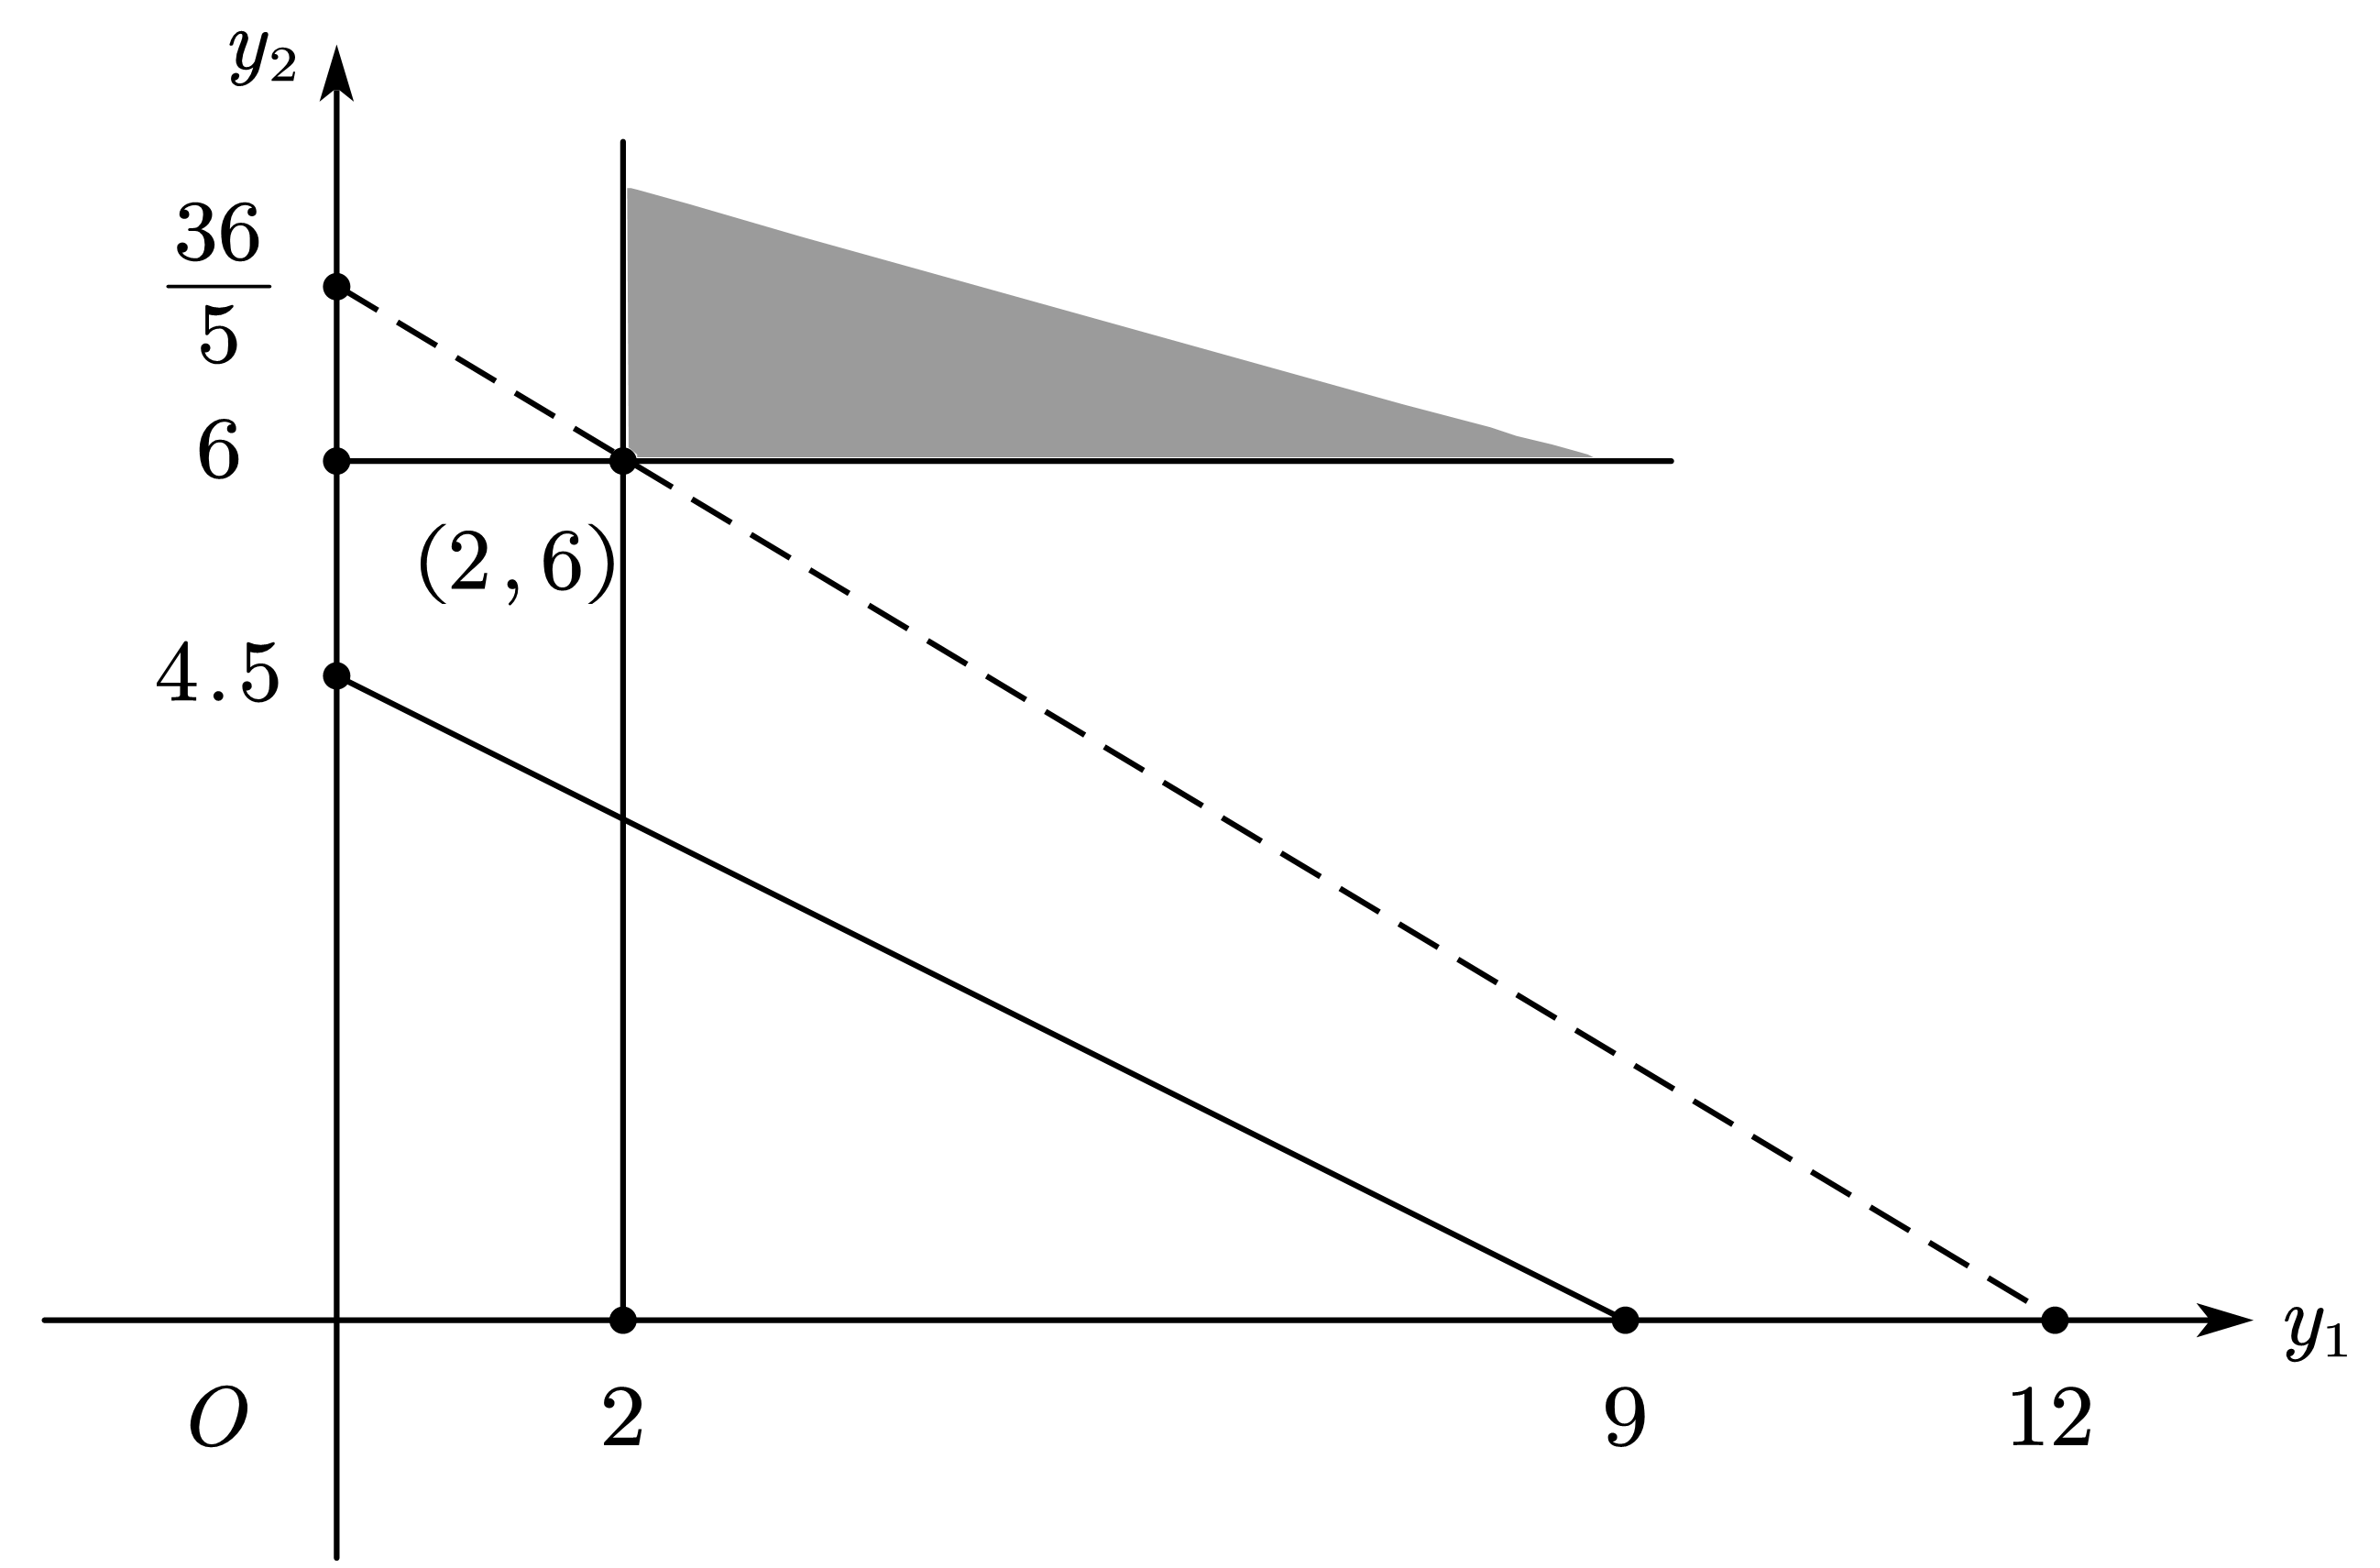
\includegraphics[width = 0.6\textwidth]{f1}
			\caption{Graphical solution}
			\label{f1}
		\end{figure}
	
	The optimal solution is at BF (2,6), i.e., $y_1=2,\ y_2=6$ with $W=36$. And the shadow prices for the resources are 2 and 6, respectively.
	\end{solution}
	
\end{enumerate}

\item Consider the following problem.

Maximize $$Z=2x_1-4x_2$$
subject to
\begin{equation*}
\begin{aligned}
x_1-x_2&\ls 1\\
x_1,x_2&\gs 0\\
\end{aligned}
\end{equation*}
\begin{enumerate}
	\item Construct the dual problem, and then find its optimal solution by inspection.
	
	\begin{solution}
		The dual problem is:
		
		Minimize $$W=y_1$$
		subject to
		\begin{equation*}
		\begin{aligned}
		y_1&\gs 2\\
		-y_1&\gs -4\\
		y_1&\gs 0\\
		\end{aligned}
		\end{equation*}
		
		Simplify the constraints, we get $2\ls y_1\ls 4$. Since we should minimize $W=y_1$, the optimal solution is $y_1=2$ with $W=2$.
		
	\end{solution}
	
	\item Use the complementary slackness property and the optimal solution for the dual problem to find the optimal solution for the primal problem.
	
	\begin{solution}
		
		By complementary slackness property, we have
		\begin{equation*}
		\begin{aligned}
		y_1=2&\Rightarrow x_2=0\\
		x_1-x_2=1, x_2=0&\Rightarrow x_1=1\\
		\end{aligned}
		\end{equation*}
		
		Therefore, the optimal solution for primal problem is $x_1=1,\ x_2=0$ with $Z=2$.
	\end{solution}
	
\end{enumerate}

\item Consider the following problem.

Maximize $$Z=x_1+x_2$$
subject to
\begin{equation*}
\begin{aligned}
&(\text{O})\quad x_1+2x_2= 10\\
&(\text{B})\quad 2x_1+x_2\gs 2\\
&(\text{O})\quad x_1 \text{ uncontrained in sign}\\
&(\text{S})\quad x_2\gs 0\\
\end{aligned}
\end{equation*}
Use the SOB method to construct the dual problem.
\begin{solution}
	
	The dual problem is:
	
	Minimize $$W=10y_1+2y_2$$
	subject to
	\begin{equation*}
	\begin{aligned}
	&(\text{O})\quad y_1\text{ uncontrained in sign}\\
	&(\text{B})\quad y_2\ls 0\\
	&(\text{O})\quad y_1+2y_2=1\\
	&(\text{S})\quad 2y_1+y_2\gs 1\\
	\end{aligned}
	\end{equation*}
	
\end{solution}

\item Consider the following problem.

Maximize $$Z=2x_1+7x_2-3x_3$$
subject to
\begin{equation*}
\begin{aligned}
x_1+3x_2+4x_3&\ls 30\\
x_1+4x_2-x_3&\ls 10\\
x_1,x_2,x_3&\gs 0\\
\end{aligned}
\end{equation*}
By letting $x_4$ and $x_5$ be the slack variables for the respective constraints, the simplex method yields the following final set of equations:
\begin{equation*}
\begin{aligned}
(0)\qquad\ \ Z+x_2+x_3+2x_5&=20\\
(1)\quad\, -x_2+5x_3+x_4-x_5&=20\\
(2)\qquad\ x_1+4x_2-x_3+x_5&=10\\
\end{aligned}
\end{equation*}
Now you are to conduct sensitivity analysis by independently investigating each of the following three changes in the original model. For each change, use the sensitivity analysis procedure to revise this set of equations (in tableau form) and convert it to proper form from Gaussian elimination for identifying and evaluating the current basic solution. Then test this solution for feasibility and for optimality. If either test fails, reoptimize to find a new optimal solution.
\begin{enumerate}
	\item 	Change the right-hand sides to
	\begin{equation*}
	\begin{bmatrix}
	b_1\\
	b_2
	\end{bmatrix}
	=
	\begin{bmatrix}
	20\\
	30
	\end{bmatrix}
	\end{equation*}
	
	\begin{solution}
		The final set of equations in tableau form are shown in Tab.\ref{tab1}.
		\begin{table}[h]
			\centering
			\caption{Final simplex tableau}
			\label{tab1}
			\begin{tabular}{cccccccccc}
				\toprule[1.5pt]
				~&Basic Variable    &Eq.  &$Z$  &$x_1$&$x_2$&$x_3$&$x_4$&$x_5$&Right Side\\
				\midrule[0.5pt]
				\multirow{3}*{\text{Final}}
				&$Z$     &(0)  &1  &0      &1      &1       &0       &2       &20\\
				&$x_4$  &(1)  &0  &0      &$-1$ &5       &1       &$-1$  &20 \\
				&$x_1$  &(2)  &0  &1      &4      &$-1$  &0       &1       &10 \\	
				\bottomrule[1.5pt]
			\end{tabular}
		\end{table}		
		
		From the above tableau, we know that:
		\begin{equation*}
		\my^*=[0,2],\quad
		\mS^*=\begin{bmatrix}
		1&-1\\
		0&1\\
		\end{bmatrix}		
		\end{equation*}
		Therefore,
		\begin{equation*}
		\mb^*=\mS^*\cdot\overline{\mb}
		=\begin{bmatrix}
		1&-1\\
		0&1\\
		\end{bmatrix}\begin{bmatrix}
		20\\
		30\\
		\end{bmatrix}
		=\begin{bmatrix}
		-10\\
		30
		\end{bmatrix}
		\end{equation*}
		\begin{equation*}
		\mz^*=\my^*\cdot\overline{\mb}=[0,2]\begin{bmatrix}
		20\\
		30\\
		\end{bmatrix}=60
		\end{equation*}	
	Since there exists negative element in right side, we perform dual simplex method to solve this problem, shown in Tab.\ref{tab2}.
	\renewcommand\arraystretch{1.5}
	\begin{table}[h]
		\centering
		\caption{Dual simplex method tableau for changes in right side}
		\label{tab2}
		\begin{tabular}{cccccccccc}
			\toprule[1.5pt]
			~&Basic Variable    &Eq.  &$Z$  &$x_1$&$x_2$&$x_3$&$x_4$&$x_5$&Right Side\\
			\midrule[0.5pt]
			\multirow{3}*{\text{Revised}}
			&$Z$     &(0)  &1  &0      &1      &1       &0       &2       &60\\
			&$x_4$  &(1)  &0  &0      &$-1$ &5       &1       &$-1$  &$-10$ \\
			&$x_1$  &(2)  &0  &1      &4      &$-1$  &0       &1       &30 \\	
			\midrule[0.5pt]
			\multirow{3}*{\text{Iteration 1}}
			&$Z$     &(0)  &1  &1      &0      &6       &1       &1       &50\\
			&$x_2$  &(1)  &0  &0      &1      &$-5$  &$-1$  &1      &10 \\
			&$x_1$  &(2)  &0  &1      &0      &19     &4       &$-3$ &$-10$ \\	
			\midrule[0.5pt]
			\multirow{3}*{\text{Iteration 2}}
			&$Z$     &(0)  &1  &$\tfrac{4}{3}$ &0      &$\tfrac{37}{3}$      &$\tfrac{7}{3}$      &0       &$\tfrac{140}{3}$\\
			&$x_2$  &(1)  &0  &$\tfrac{1}{3}$      &1      &$\tfrac{4}{3}$&$\tfrac{1}{3}$  &0      &$\tfrac{20}{3}$\\
			&$x_5$  &(2)  &0  &$-\tfrac{1}{3}$&0      &$-\tfrac{19}{3}$&$-\tfrac{4}{3}$   &1 &$\tfrac{10}{3}$\\	
			\bottomrule[1.5pt]
		\end{tabular}
	\end{table}		
	\renewcommand\arraystretch{1}

	Therefore, the optimal solution is $x_1=0, x_2=\tfrac{20}{3},x_3=0$ with $Z=\tfrac{140}{3}$.
	\end{solution}

	\item Change the coefficients of $x_3$ to
	\begin{equation*}
	\begin{bmatrix}
	c_3\\
	a_{13}\\
	a_{23}\\
	\end{bmatrix}
	=
	\begin{bmatrix}
	-2\\
	3\\
	-2\\
	\end{bmatrix}
	\end{equation*}
	\begin{solution}
		$x_3$ is a nonbasic variable and we know that
		\begin{equation*}
		\mz_3^*-\overline{\mc}_3=\my^*\cdot\overline{\mA}_3-\overline{\mc}_3
		=[0,2]\begin{bmatrix}
		3\\
		-2\\
		\end{bmatrix}+2=-2
		\end{equation*}
		\begin{equation*}
		\mA_3^*=\mS^*\cdot\overline{\mA}_3=\begin{bmatrix}
		1&-1\\
		0&1\\
		\end{bmatrix}\begin{bmatrix}
		3\\
		-2
		\end{bmatrix}=\begin{bmatrix}
		5\\
		-2
		\end{bmatrix}
		\end{equation*}
		Since there exists negative element in row 0, we perform simplex method to solve this problem, shown in Tab.\ref{tab3}.
		\renewcommand\arraystretch{1.5}
		\begin{table}[h]
			\centering
			\caption{Simplex method tableau for changes in nonbasic variable}
			\label{tab3}
			\begin{tabular}{cccccccccc}
				\toprule[1.5pt]
				~&Basic Variable    &Eq.  &$Z$  &$x_1$&$x_2$&$x_3$&$x_4$&$x_5$&Right Side\\
				\midrule[0.5pt]
				\multirow{3}*{\text{Revised}}
				&$Z$     &(0)  &1  &0      &1      &$-2$ &0       &2       &20\\
				&$x_4$  &(1)  &0  &0      &$-1$ &5       &1       &$-1$  &20 \\
				&$x_1$  &(2)  &0  &1      &4      &$-2$  &0       &1       &10 \\	
				\midrule[0.5pt]
				\multirow{3}*{\text{Iteration 1}}
				&$Z$     &(0)  &1  &1      &$\tfrac{3}{5}$&0       &$\tfrac{2}{5}$&$\tfrac{8}{5}$&28\\
				&$x_3$  &(1)  &0  &0      &$-\tfrac{1}{5}$&1  &$\tfrac{1}{5}$&$-\tfrac{1}{5}$&4 \\
				&$x_1$  &(2)  &0  &1      &$\tfrac{18}{5}$&0&$\tfrac{2}{5}$&$\tfrac{3}{5}$ &18 \\		
				\bottomrule[1.5pt]
			\end{tabular}
		\end{table}
	\renewcommand\arraystretch{1}		
		
		Therefore, the optimal solution is $x_1=18, x_2=0,x_3=4$ with $Z=28$.
		
	\end{solution}
	\item Change the coefficients of $x_1$ to
	\begin{equation*}
	\begin{bmatrix}
	c_1\\
	a_{11}\\
	a_{21}\\
	\end{bmatrix}
	=
	\begin{bmatrix}
	4\\
	3\\
	2\\
	\end{bmatrix}
	\end{equation*}
	\begin{solution}
		$x_1$ is a basic variable and we know that
		\begin{equation*}
		\mz_1^*-\overline{\mc}_1=\my^*\cdot\overline{\mA}_1-\overline{\mc}_1
		=[0,2]\begin{bmatrix}
		3\\
		2\\
		\end{bmatrix}-4=0
		\end{equation*}
		\begin{equation*}
		\mA_1^*=\mS^*\cdot\overline{\mA}_1=\begin{bmatrix}
		1&-1\\
		0&1\\
		\end{bmatrix}\begin{bmatrix}
		3\\
		2
		\end{bmatrix}=\begin{bmatrix}
		1\\
		2
		\end{bmatrix}
		\end{equation*}
		Convert this problem into proper form, shown in Tab.\ref{tab4}.
		\renewcommand\arraystretch{1.5}
		\begin{table}[h]
			\centering
			\caption{Simplex method tableau for changes in basic variable}
			\label{tab4}
			\begin{tabular}{cccccccccc}
				\toprule[1.5pt]
				~&Basic Variable    &Eq.  &$Z$  &$x_1$&$x_2$&$x_3$&$x_4$&$x_5$&Right Side\\
				\midrule[0.5pt]
				\multirow{3}*{\text{Revised}}
				&$Z$     &(0)  &1  &0      &1      &1      &0       &2       &20\\
				&$x_4$  &(1)  &0  &1      &$-1$ &5       &1       &$-1$  &20 \\
				&$x_1$  &(2)  &0  &2      &4      &$-1$  &0       &1       &10 \\	
				\midrule[0.5pt]
				\multirow{3}*{\text{Proper Form}}
				&$Z$     &(0)  &1  &0      &1     &1      &0&2&20\\
				&$x_4$  &(1)  &0  &0      &$-3$&$\tfrac{11}{2}$ &1       &$-\tfrac{3}{2}$&15\\
				&$x_1$  &(2)  &0  &1      &2&$-\tfrac{1}{2}$&0&$\tfrac{1}{2}$&5 \\		
				\bottomrule[1.5pt]
			\end{tabular}
		\end{table}
		\renewcommand\arraystretch{1}
		
		Since it already satisfies optimality test and feasibility test, the optimal solution is $x_1=5,x_2=0,x_3=0$ with $Z=20$.
	\end{solution}
		
\end{enumerate}

\item 	Consider the following problem.

Maximize $$Z=c_1x_1+c_2x_2$$
subject to
\begin{equation*}
\begin{aligned}
2x_1-x_2&\ls b_1\\
x_1-x_2&\ls b_2\\
x_1,x_2&\gs 0\\
\end{aligned}
\end{equation*}
Let $x_3$ and $x_4$ denote the slack variables for the respective functional constraints. When $c_1 =3, c_2= -2, b_1=30$, and $b_2=10$, the simplex method yields the following final simplex tableau.
\begin{table}[h]
	\centering
	\caption{Final simplex tableau}
	\label{tab5}
	\begin{tabular}{ccccccccc}
		\toprule[1.5pt]
		~&Basic Variable    &Eq.  &$Z$  &$x_1$&$x_2$&$x_3$&$x_4$&Right Side\\
		\midrule[0.5pt]
		\multirow{3}*{\text{Final}}
		&$Z$     &(0)  &1  &0      &0      &1       &1        &40\\
		&$x_2$  &(1)  &0  &0      &1      &1       &$-2$   &10 \\
		&$x_1$  &(2)  &0  &1      &0      &1       &$-1$   &20 \\	
		\bottomrule[1.5pt]
	\end{tabular}
\end{table}

\begin{enumerate}
	\item Determine the allowable range for $c_1$.
	\begin{solution}
		Increment $c_1=3$ by $\Delta c_1$, which changes row 0 to
		\begin{equation*}
		\text{Row 0}=[-\Delta c_1,0,1,1,40]
		\end{equation*}
		Perform elementary row operations to restore proper form from Gaussian elimination:
		\begin{equation*}
			\text{New row 0}=[0,0,1+\Delta c_1,1-\Delta c_1,40+20\Delta c_1]
		\end{equation*}
		Keep the coefficients of the nonbasic variables nonnegative:
		\begin{equation*}
		\begin{aligned}
		1+\Delta c_1\gs 0&\Rightarrow\Delta c_1\gs-1,\\
		1-\Delta c_1\gs 0&\Rightarrow\Delta c_1\ls 1\\
		\end{aligned}
		\end{equation*}
		Since $c_1=3+\Delta c_1$, the allowable range for $c_1$ is
		\begin{equation*}
		2\ls c_1 \ls 4
		\end{equation*}
	\end{solution}	
\vspace*{-0.5cm}	
	\item Determine the allowable range for $b_1$.
	\begin{solution}
		Increment $b_1=30$ by $\Delta b_1$, we get
		\begin{equation*}
		\mb^*=\mS^*\cdot\overline{\mb}=\begin{bmatrix}
		1&-2\\
		1&-1\\
		\end{bmatrix}\begin{bmatrix}
		30+\Delta b_1\\
		10\\
		\end{bmatrix}
		=\begin{bmatrix}
		10+\Delta b_1\\
		20+\Delta b_1\\
		\end{bmatrix}
		\end{equation*}
		Keep the coefficients of right side nonnegative:
		\begin{equation*}
		\begin{aligned}
		10+\Delta b_1\gs 0&\Rightarrow\Delta b_1\gs -10,\\
		20+\Delta b_1\gs 0&\Rightarrow\Delta b_1\gs  -20\\
		\end{aligned}		
		\end{equation*}
		Since $b_1=30+\Delta b_1$, the allowable range for $b_1$ is
		\begin{equation*}
		b_1\gs 20
		\end{equation*}
	\end{solution}
\end{enumerate}

% w.r.t the external
\end{enumerate}
%  The source code to plot Figure \ref{fig:1} could be found in Appendix \ref{sec:a:code}. Here are the core codes:
%  \lstinputlisting[firstline=6,lastline=7, firstnumber=6]{matlabscript.m}

%  \newpage
%  \appendix
%  \section{Source code}
%  \label{sec:a:code}
%  % \lstlistoflistings
%  Source code for plotting Figure \ref{fig:1} is shown as follows.
%  \lstinputlisting[caption=FigurePlot]{matlabscript.m}
  
\end{document}
